\section{Waves}

In this lab you will use software to model wave motion.
\hfill \break

\underline{\textbf{Part 1}} \par
At $t = 0$ a wave is given by
\begin{equation}
y(x) = 1.6e^{-0.75x^2} + e^{-0.5(x-3)^2}
\end{equation}
and moves to the right with speed $v$.
Choose a value for $v$ (anything besides 5 m/s since that is used in the example figure below) and create a plot showing the wave at $t =$ 0, 1, and 2 s.
\begin{figure}[H]
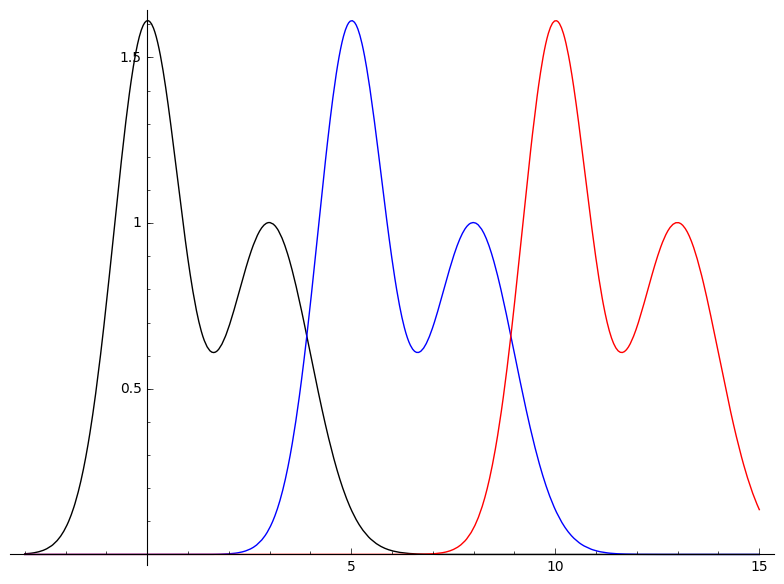
\includegraphics[scale=0.50]{figures/waves/fig1.png}
\end{figure}
Do this by modifying the SageMath starter code below.
\begin{verbatim}
y1, y2, y3, x = var("y1, y2, y3, x")

y1 = x + 1
y2 = x^2
y3 = x^3 - 1

p1 = plot(y1, (x, -2, 2), color="black")
p2 = plot(y2, (x, -2, 2), color="blue")
p3 = plot(y3, (x, -2, 2), color="red")

g = Graphics()
g += p1
g += p2
g += p3
g.show()
\end{verbatim}

\underline{\textbf{Part 2}} \par
Now create an animated version of the plot from part 1.
Save the animated .gif file and upload it to GitHub when you submit your lab.
Use the code below as a starting point.
\begin{verbatim}
traveling_wave = [plot(exp(-(x - t)^2), (-1, 4), ymin=0, ymax=2) for t in sxrange(0, 5, 0.1)]
animation = animate(traveling_wave)
animation.show(delay=10)
\end{verbatim}

\underline{\textbf{Part 3}} \par
Create an animation of a right-moving wave interfering with a left-moving wave.

\pagebreak \clearpage
